\chapter{Solutions SDN disponibles}

Le but de ce chapitre n'est pas de détailler chaque solution SDN émergente, mais d'analyser les offres des principaux constructeurs du marché et leur positionnement pour les tendances qu'on peut attendre de SDN prochainement.
Mais d'abord il propose un point sur la situation de SDN, en présentant comment les organisations supportant SDN se sont positionnées pour le développement de standards et de protocoles.



%https://www.opennetworking.org/sdn-resources/onf-products-listing

\section{Un point sur la situation}
%\subsection{ONF}

%The Open Networking Foundation (ONF) is a non‑profit, user‑driven organization dedicated to accelerating the adoption of open Software‑Defined Networking (SDN). We view SDN as a disruptive approach to networking that will change how virtually every company with a network operates.

%Launched in 2011 by Deutsche Telekom, Facebook, Google, Microsoft, Verizon, and Yahoo!, ONF is a nonprofit organization dedicated to rethinking networking, and quickly and collaboratively bringing to market SDN standards and solutions. ONF is accelerating the delivery and commercialization of SDN and fostering a vibrant market of products, services, applications, customers, and users. 


Open Networking Foudation (\gls{onf}) est une organisation non lucrative et axée sur l'utilisateur, dédiée à l'accélération de l'adoption ouverte de SDN. Cette organisation voit SDN comme une approche réseau qui va changer la façon dont chaque entreprise opère un réseau.
\gls{onf} a été initiée en 2011 par Deutsche Telekom, Facebook, Google, Microsoft, Verizon et Yahoo dans le but de travailler en collaboration pour repenser les réseaux informatiques et apporter rapidement au marché les solutions et les standards SDN. Avec la coopération de grands experts mondiaux, ONF accélère la commercialisation de SDN en favorisant un  marché dynamique de produits, de services, d'applications, de clients et d'utilisateurs. ONF compte aujourd'hui plus de 100 entreprises membres collaboratives, de toute taille et variété. \cite{ONFOverview}

\gls{onf} s'est fortement impliqué pour standardiser le protocole \gls{openflow}. Ce protocole se focalise sur la standardisation des interfaces entre les applications et le contrôleur et les interfaces entre le contrôleur et l'équipement de commutation. De grands noms de l'industrie (comme Cisco, Microsoft, Google etc.) ont réalisé des produits supportant OpenFlow, comme des switches. \cite{SurveySDNArchi} %Dans l'image \ref{imgArchi} on voit l'architecture SDN avec les interfaces que OpenFlow essai de définir.



%The Open Network Foundation (ONF) [3] has been trying to standardize the OpenFlow protocol. As the control plane abstracts network applications from underlying hardware infrastructure, they focus on standardizing the inter- faces between: (1) network applications and the controller (i.e. northbound interface) and (2) the controller and the switching infrastructure (i.e., southbound interface) which defines the OpenFlow protocol itself. 
%Many large companies (such as Cisco, Microsoft, Google, etc.) have produced OpenFlow-supported products (such as switches).

Le fort soutien de l'industrie, de la recherche et des académies que \gls{onf} et sa proposition de \gls{sdn}, \gls{openflow}, ont pu recueillir est assez révélateur. Les résultats dans ces différents secteurs ont produit un nombre significatif de livrables dans la forme d'articles de recherche, d'implémentations de logiciels de référence et même de hardware. Il y a eu également des efforts de standardisation de SDN de la part d'autres organisations produisant des normes, comme IETF et IRTF. \cite{SurveySDNIntro}
%The strong support from industry, research, and academia that the Open Networking Foundation (ONF) and its SDN proposal, OpenFlow, has been able to gather is quite impres- sive. The resulting critical mass from these different sectors has produced a significant number of deliverables in the form of research papers, reference software implementations, and even hardware. So much so that some argue that OpenFlow’s SDN architecture is the current SDN de-facto standard. In line with this trend, the remainder of this section focuses on OpenFlow’s SDN model. 

%On the academic side, the OpenFlow Network Research Center [4] has been created with a focus on SDN research. There have also been standardization efforts on SDN at the IETF and IRTF and other standards producing organizations.

%\section{Solution logiciel open source OpenDaylight}
%The Linux Foundation and—in its OpenDay- light Project—has introduced a community-led and industry-supported open source framework to accelerate SDN adoption, foster new innovation, and give it a more open and transparent approach.
%OpenDaylight has the support it needs to transform SDN. Big Switch Networks, Brocade, Cisco, Citrix, Ericsson, IBM, Juniper Networks, Microsoft, NEC, Red Hat, and VMware are all founding Platinum and Gold members of the project. It will donate software and engineering resources for this open source framework, and help define the future of an open SDN platform. Yes, that’s right: Cisco and Juniper, Microsoft and Red Hat, and other major industry rivals are all joining forces.

La fondation Linux avec son projet \gls{opendaylight} a introduit une plateforme \gls{opensource} guidée par la communauté et supportée par l'industrie. Le but du projet est d'accélérer l'adoption de SDN, d'encourager l'innovation et de présenter une approche plus ouverte et transparente. OpenDaylight a le soutien dont il a besoin pour transformer SDN. Big Switch Networks, Brocade, Cisco, Citrix, Ericsson, IBM, Juniper Networks, Microsoft, NEC, Red Hat et VMware sont tous des fondateurs Platinum et membres Gold du projet. Ces acteurs vont apporter des ressources d'ingénierie logicielle et vont aider à définir le futur de cette plateforme SDN ouverte. Le point important à noter est l'union de forces des rivaux de l'industrie. \cite{ExecutiveGuideToSDNLinux}



%\subsection{OpenFlow - Protocoles standardisés}
%\section{Dispositifs de commutation}
%The basic idea is simple: we exploit the fact that most modern Ethernet switches and routers contain flow-tables (typically built from TCAMs) that run at line-rate to im- plement firewalls, NAT, QoS, and to collect statistics. While each vendor’s flow-table is different, we’ve identified an in- teresting common set of functions that run in many switches and routers. OpenFlow exploits this common set of func- tions.




%\section{Contrôleur}
%Controllers. A controller adds and removes flow-entries from the Flow Table on behalf of experiments. For example, a static controller might be a simple application running on a PC to statically establish flows to interconnect a set of test computers for the duration of an experiment. In this case the flows resemble VLANs in current networks— providing a simple mechanism to isolate experimental traffic from the production network. Viewed this way, OpenFlow is a generalization of VLANs.


%Many companies are offering a wide array of SDN products. However, each SDN product strategy can differ radically from company to company. While some base their products on the traditional view of SDN, others offer software overlays with hypervisors that control the virtual network.
Diverses entreprises offrent une large gamme de produits SDN. Toutefois, les stratégies de chaque produit SDN peuvent différer radicalement selon les sociétés. Alors que certaines basent leurs produits dans l'optique traditionnelle de SDN, d'autres proposent leurs propres visions et offrent des produits en rapport. Un article sur SearchSDN \cite{42Vendors} propose une liste représentative des principaux vendeurs. ONF divulgue une liste de produits SDN soumis par ces membres \cite{ProductDirectory}.  

Les catégories des produits varient aussi en fonction du secteur d'activité des sociétés qui les offrent. En général, les commerçants de chips/silicium proposent des processeurs optimisant la performance du hardware de commutation.  Les vendeurs de switches offrent du matériel capable de communiquer avec un contrôleur SDN. Les spécialistes de la \gls{virtualisation} offrent des solutions logicielles simulant de switchs ou routeurs SDN virtualisés. D'autres sociétés vont investir sur le développement d'un contrôleur SDN. Une pratique adoptée par les géants de l'industrie est l'offre de tout l'écosystème SDN avec souvent un accent sur des applications pour l'automatisation de \gls{datacenter}.\cite{2013GuideSDNNVEcosystem} L'image \ref{imgArchi} montre l'architecture de base SDN qui peut être très proche de certaines solutions ou assez différente selon la stratégie du vendeur.
 
\begin{figure}[!h] %on ouvre l'environnement figure
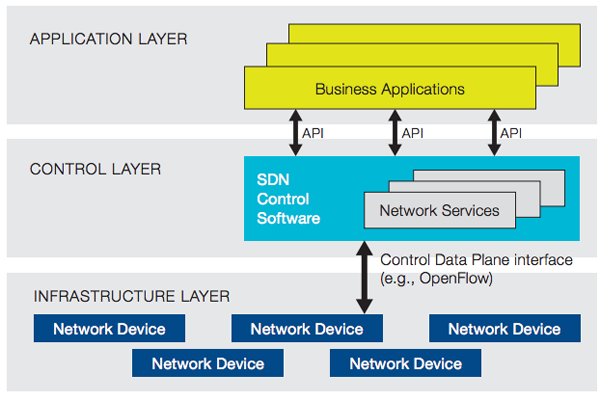
\includegraphics[width=15cm]{images/openflowArchi.png} %ou image.png, .jpeg etc.
\caption{ Architecture OpenFlow SDN par ONF \cite{SDNNewNormONFExecutiveSummary}} %la légende
\label{imgArchi} %l'étiquette pour faire référence à cette image
\end{figure} %on ferme l'environnement figure
 
Le tableau ci-dessous identifie les principaux produits SDN et les sociétés les plus représentatives leur fournissent.

\begin{table}[!h]
\centering
\begin{tabular}{|p{6cm}|p{9cm}|}
\hline 
\bf Produit & \bf Vendeur \\ 
\hline 
Chips pour matériel réseau & Boradcom, Intel, Marvell, Mellanox \\ 
\hline 
Switches SDN & Alcatel-Lucent, Avaya, Cisco, Dell, Extreme Networks, HP, NEC, PICA-8, IBM \\ 
\hline 
Systèmes pour le management et automatisation du réseau & Packet Design, QualiSystems, EMC, NetScout, CA, HP \\ 
\hline 
Services réseau avec SDN & Embrane, A10, Radware, HP, Riverbed, Citrix, Cisco,  Extreme Networks, NEC \\ 
\hline 
Outils pour la réalisation de tests, les propres résultats des tests & QualiSystems, inCNTRE, Ixia, Spirent \\ 
\hline 
Standards et protocoles & ONF, IEEE, IETF \\ 
\hline 
Contrôleur SDN & Big Switch Networks, NEC, Nuage Networks, Netsocket, HP, Cisco, Open Daylight Consortium, VMware/Nicira \\ 
\hline 
Switchs virtuels et APIs & Citrix, Microsoft, VMWare, Big Switch Networks, Cisco \\ 
\hline 
\end{tabular} 
\caption{Produits SDN et les principaux fournisseurs \cite{2013GuideSDNNVEcosystem}}
\end{table} 
 
Ensuite ce document présente les principales solutions construites par les plus importants vendeurs du marché.

%%%%%%%Pas exhaustif>>>


\section{Écosystème SDN HP, gamme de solutions virtualisées Data Center}

%Hewlett-Packard executives outlined their software-defined networking (SDN) strategy and position in the market and made a few bets on when the technology will go mainstream. The bet: SDNs will be deployed enterprise-wide in 2015 and represent a \$2 billion market in 2016.
%HP’s argument is that its specialty in automating the data center, as well as a large footprint of customers, make it a leading SDN player.

Les dirigeants de Hewlett-Packard exposent les grandes lignes pour leur stratégie SDN et leur position face au marché, en pariant sur l'adoption dominante de cette technologie. HP espère que SDN sera largement déployé dans les entreprises en 2015 et qu'il représentera un marché de 2 milliards de dollars en 2016. La société investit dans sa spécialité d'automatisation de \gls{datacenter} pour argumenter sa position d'acteur SDN en premier plan. \cite{ExecutiveGuideToSDNHP}


HP a récemment annoncé sa nouvelle gamme de solutions SDN. Avec l'architecture réseau convergé FlexNetwork, HP se vante d'offrir jusqu'à deux fois plus d'évolutivité avec 75\% de complexité en moins, par comparaison à d'autres solutions "fabric" proposées sur le marché. En outre, HP affirme que sa solution \gls{fabric} va réduire les délais d’approvisionnement de \gls{datacenter} de quelques mois à seulement quelques minutes. Le portfolio des services SDN proposés par HP est assez solide, avec des produits ciblant différents points qui vont du traitement des infrastructures existantes à la simplification d'opérations. Par exemple, le HP Virtualized Services Router a été conçu pour éliminer le hardware pouvant être remplacé par des services dans les \glspl{vm}.  

%Hewlett-Packard is stepping up its data center game with a recent announcement of a new suite of solutions for software-defined networking. Built on its FlexNetwork converged networking architecture, HP boasts that it can offer up to two times greater scalability with “75 percent less complexity” compared to other networking fabrics on the market. Furthermore, HP asserted that its data center fabric will reduce provisioning timeframes all the way down from months to mere minutes.


%HP’s portfolio of SDN services is quite substantial, with products aimed at addressing various issues, from dealing with legacy infrastructures to simplifying operations. For example, the HP Virtualized Services Router is designed to cut back data center footprints by delivering services on a virtual machine, which should eliminate “unnecessary hardware.” In addition, the HP HSR 6800 Router Series aims to simplify network service delivery by consolidating routing, firewall, switching, and security onto one device that supports thousands of users. HP’s suite of SDN offerings will be rolling out over the course of the year. Only the HSR 6800 Router Series is available worldwide now, and it holds a starting price of \$46,000. 

La suite d'offres SDN de HP est assez importante, avec des produits qui ciblent divers domaines, l'interopérabilité avec les infrastructures traditionnelles et la simplification des opérations. Par exemple, le produit "HP Virtualized Services Router" est conçu pour éliminer du matériel non essentiel dans les \glspl{datacenter}. De plus, la série "HP HSR 6800 Router Series" a pour but de simplifier la livraison de service réseau en consolidant les fonctions des routage, commutation et sécurité sur le même dispositif supportant des milliers d'utilisateurs. "HP HSR 6800 Router Series" est disponible mondialement au prix initial de \$46,000. \cite{ExecutiveGuideToSDNHPFabric}


%SDN Dev Center.
%SDN App Store.
%HP SDN Developer Kit

\section{Cisco ONE, hardware programmable}

%Cisco also announced it will spend up to \$863 million to acquire Insieme Networks, the company Cisco formed more than a year ago to develop data center networks that are programmable and flexible enough to keep up with the cloud and heavily virtualized data centers.

%The result of Insieme’s work is the Application Centric Infrastructure (ACI), which includes a new line of Nexus 9000 switches that form an application-aware switching fabric along with a centralized controller that manages both virtual and physical network infrastructures.



Cisco a annoncé en novembre 2013 \gls{aci} soutenue par l'investissement de 863 millions de dollars pour l'acquisition de Insieme Networks. La start-up développe des réseaux programmables et flexibles pour le cloud et les data centers hautement virtualisés. \gls{aci} est une architecture holistique pour l'automatisation de profiles d'application dirigés par politiques centralisés. Le but est d'apporter flexibilité aux logiciels avec "scalibility" et performance hardware. 


La solution concrétise \gls{one}. Annoncée précédemment, \gls{one} est une solution complète pour aider les réseaux à devenir plus ouverts, programmables et sensibles aux applications. L'offre inclut une nouvelle ligne de 9000 switches avec un contrôleur capable de gérer les infrastructures physiques et virtuelles. \gls{aci} est disponible sur le marché pour \$75000 avec 288 ports. \cite{CiscoInsiemeLast}


%For now, customers can get into ACI for as low as \$75,000 for 288 ports with a pay-as-you-grow model, said Chambers.


Cisco estime qu'une compréhension approfondie de la couche matérielle est nécessaire. Cela veut dire à la fois que le logiciel et le matériel devraient être développés par la même entreprise et reliés entre eux. À cet effet, Cisco a cherché à embarquer des logiciels très sophistiqués dans ses switches dans le but de renforcer sa crédibilité SDN.
%with centralized automation and policy-driven application profiles. ACI delivers software flexibility with the scalability of hardware performance.
Alors que cette stratégie ne concorde pas tout à fait avec la définition de SDN par \gls{onf}, le résultat obtenu est proche : les switches devient plus manageables à travers une interface centrale fournie. Cisco désigne ce modèle comme réseau centré sur les applications, parce que l'organisation introduit des \glspl{api} qui permettent aux applications d'interagir directement avec le réseau. \cite{CiscoSDNONE}

%Cisco refers to this as “application-centric networking” because the company is introducing programmable APIs that allow apps to draw intelligence (and value) directly from the network itself.

%Cisco Open Network Environment (ONE) is a comprehensive solution to help networks become more open, programmable, and application-aware. The broad capabilities of Cisco ONE help meet the needs of numerous market segments, including emerging concepts such as software-defined networking (SDN).

%Cisco believes a thorough understanding of the hardware layer is needed. In turn, this means the software and hardware should be developed by the same company and linked together. To that end, Cisco has so far sought to boost its SDN credibility by embedding more sophisticated software in its switches. While this doesn’t fit the exact definition of SDN—which moves control from switches up into a central management plane, probably using some form of commodity x86 server—it has roughly the same outcome. Switches become more manageable via a central interface.

Cette vision suggère que Cisco tient à s'assurer que cette approche axée logiciel ne menace pas son business consolidé du marché de hardware réseau. D'un côté cela permet de maintenir les prix élevés de ces équipements réseau "smarts" tout en permettant de fournir les capacités SDN. Cette approche indique que l'organisation compte embarquer les informations sur les réseaux à partir du matériel vers un logiciel de contrôle plus flexible. Cela diffère de l'approche fédérée par \gls{onf} dont les informations sont diffusées en sens inverse. 

%Cisco’s view, it suggests the company is keen to make sure a more software-focused approach does not threaten its longstanding networking hardware business. For one thing, it lets Cisco keep the prices high on its networking equipment: By using its Cisco ONE (Open Network Environment) technologies to put more software on its switches, it can give customers SDN features while encouraging them to keep on buying its “smart” equipment, which is priced at a premium.

%The approach means Cisco wants to embed information about the network at the hardware layer and have it flow up to a more flexible software control plane. This differs from the approach taken by SDN-like tech- nologies such as OpenFlow and Nicira, which see intelligence originate and reside in the control plane, with decisions pushed out to the hardware.

Finalement, la proposition de Cisco semble jouable pour les investisseurs mais potentiellement inintéressante pour l'innovation. Il est probable que l'entreprise utilise son poids pour renforcer sa vision particulière de SDN en tant qu'un standard. Si cela se produit, les entreprises devront continuer à dépenser de grandes sommes sur du matériel et logiciel propriétaires. Bien que ce scénario puisse rendre SDN plus accessible au début, il risque de devenir contraignant dans le futur. \cite{ExecutiveGuideToSDNCisco}

%Ultimately, Cisco’s approach is good for investors but potentially bad for innovation, as the company will likely seek to use its influence to make its particular view of SDN the industry standard. If this happens, businesses will have to keep spending large amounts of money on IT equipment that dovetails into proprietary software, which then has API compatibility or NIC-support for OpenFlow. Though this may make SDN slightly more ac- cessible to smaller businesses, it could lead to larger companies giving Cisco the cold shoulder and taking the Google route.



\section{Virtualisation : Big Switch Controller et VMWare NSX}

Au sein des vendeurs les plus grands et reconnus, il se peut que l'innovation soit plus difficile à atteindre. Ces entreprises ont déjà un modèle de business habituel à maintenir, ce qui est souvent contraignant pour le développement d'une technologie qui est véritablement nouvelle et différente. Pour cette raison SDN a engendré un certain nombre de start-ups avec des technologies porteuses. N'ayant pas cette contrainte, les start-ups spécialisés sur SDN ont eu la liberté de penser au réseau différemment et apporter des produits plus originaux et innovants. Les start-ups dirigent certainement le 'quand' et le 'comment' des innovations sur les réseaux programmables. \cite{startupsSDN}

%SDN has spawned a number of startups with promising technology. The reason for this is that innovation can be harder to come by in the larger, established vendors. The bureaucracy of an established vendor often burdens development teams and can make it nearly impossible to lead with technology that is truly new and different. In addition, large vendors have a customary business model to sustain and shareholders to satisfy each and every quarter. For example, its bottom line is impacted by its ability to push network hardware out the door. Therefore, the SDN strategy focuses on adding new capabilities to that hardware, as that's the least disruptive way to satisfy market demand for SDN without disrupting hardware sales.

%Startup companies have no such inertia. Startups specializing in SDN have exercised their freedom to think about networking in unusual ways and release products that are genuinely new and different. The startups are definitely leading the way when it comes to networking innovation.



Les acquisitions de ces start-ups par les leaders du marché sont devenues assez courantes. VMWare présente sa solution NSX comme une plateforme de virtualisation du réseau pour "software-defined data center". La société a investi 1,3 milliard de dollars dans l'acquisition de Nicira, une entreprise spécialisée dans la virtualisation réseau.
VMWare a intégré sa virtualisation à la technologie Nicira pour faire transiter l'information entre et autour des data centers. L'approche de Nicira est indépendante du hardware et donc capable de fonctionner comme un contrôleur dans le style SDN. Toutefois, les produits Nicira sont conçus pour gérer les réseaux virtuels plutôt que physiques. \cite{ExecutiveGuideToSDNBigSwitch}


Son principal concurrent est le Big Network Controller, un contrôleur SDN développé par la start-up Big Switch Networks. L'entreprise vise une importante part de marché et s'est fait remarquer par des grands noms. Big Switch a annoncé en novembre son premier produit, un écosystème SDN permettant aux consommateurs de modifier leurs réseaux et data centers via software. La solution est plus large que VMWare NSX et peut menacer aussi le business de fabricants d'équipement réseau, comme Cisco. \cite{BigSwitchLaunchesFirst}
%VMware NSX™ is the network virtualization and security platform for the software-defined data center. NSX brings virtualization to your existing network and transforms network operations and economics. 

%The partners will develop software defined networking (SDN) and network virtualization applications with Big Switch, and will coordinate direct sales efforts with the startup.ranging from traditional network hardware players like Juniper Networks, Arista, Brocade and HP, to hypervisor companies like Citrix and Microsoft

Dans son annonce Big Switch a révélé 27 vendeurs partenaires qui vont développer SDN et des applications virtualisées et coordonner les efforts de ventes directes avec la start-up. Les partenaires varient des traditionnels fabricants de hardware réseau comme Juniper, Brocade et HP à des fabricants d'hyperviseurs comme Citrix et Microsoft. La plateforme proposée offre \gls{fabric} switch OpenFlow qui peut exécuter dans un switch physique ou dans un hyperviseur et permet une large variété d'applications SDN, y compris la virtualisation de data center et réseau ainsi que leur monitoring. \cite{BigSwitchAnnouncement}

%Big Switch Networks is the leader in open source Software-Defined Networking (SDN) products, delivering unmatched network agility, automated network provisioning, and dramatic reductions in the cost of network operations. The company’s Open SDN™ platform offers an OpenFlow switch fabric that can run on bare metal switches and hypervisor virtual switches, and enables a wide variety of SDN network applications including data center network virtualization and network monitoring. 

%VMware made a splash with its acquisition of Nicira, and SDN acquisitions have become common.
%VMware has acquired network virtualisation company Nicira for \$1.3bn.

%VMware is expected to integrate Nicira’s technology with its virtualisation software to help move information around and between data centers. Crucially, Nicira’s approach does not care about the underlying hardware. This means that Nicira-based networks are not tied to any one supplier and are capable of an SDN-style central control plane.

%Nicira’s products are designed to manage virtual networks rather than physical ones.




%\section{Brocade Ethernet Fabric, Fibre Channel support over Ethernet}
%Virtual Cluster Switching
%Pour les architectes du réseau et serveurs de data centre.


%\section{Juniper MetaFabric Architecture}

%\section{Citrix NetScaler, plate-forme ouverte dirigée par app }
